\documentclass[10pt]{article}
\usepackage[sort]{natbib}
\usepackage{parskip}
\usepackage{mathptmx}     
\usepackage{latexsym}
\usepackage{bm,amsmath,bbm,amsfonts,nicefrac,latexsym,amsmath,amsfonts,amsbsy,amscd,amsxtra,amsgen,amsopn,bbm,amsthm,amssymb,graphicx, pbox, fixltx2e}
\usepackage{fancyhdr}
\usepackage[margin=0.8in]{geometry}
\bibliographystyle{abbrvnat}

\title{Day/Night observation operator for DALEC2 model}
\author{Ewan Pinnington}

\newtheorem{theorem}{Theorem}[section]
\newtheorem*{defn}{Definition}


\begin{document}

\maketitle

The DALEC2 model is a simple process-based model describing the carbon balance of a forest ecosystem \citep{Bloom2015} and is the new version of the original DALEC \citep{williams2005improved}. The model is constructed of six carbon pools (labile ($C_{lab}$), foliage ($C_f$), fine roots ($C_r$), woody stems and coarse roots ($C_w$), fresh leaf and fine root litter ($C_l$) and soil organic matter and coarse woody debris ($C_s$)) linked via fluxes. The aggregated canopy model (ACM) \citep{williams1997predicting} is used to calculate daily Gross Primary Production ($GPP$) of the forest, taking meteorological driving data and the modelled leaf area index (a function of $C_f$) as arguments. Figure~\ref{fig:DALEC_mod} shows a schematic of how the carbon pools are linked in DALEC2.   

\begin{figure}[ht]
    \centering
    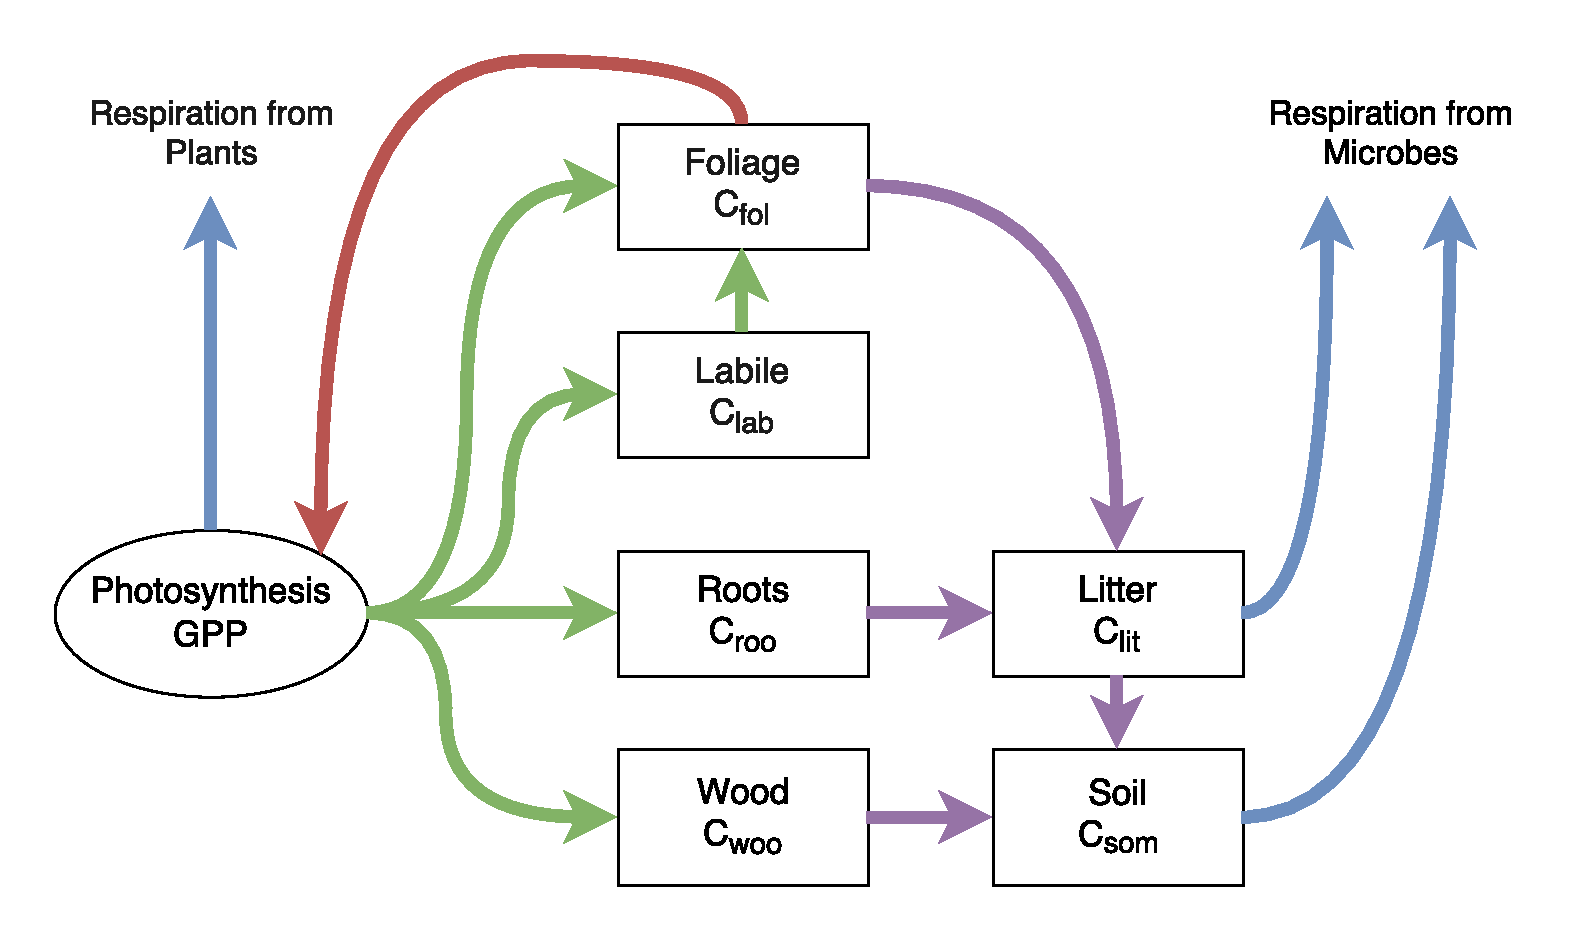
\includegraphics[width=0.5\textwidth]{dalec2diag.pdf}
    \caption{Representation of the fluxes in the DALEC2 carbon balance model. Green arrows represent C allocation, purple arrows represent litter fall and decomposition fluxes, blue arrows represent respiration fluxes and the red arrow represents the influence of leaf area index in the $GPP$ function.} \label{fig:DALEC_mod}
\end{figure}

The model equations for the carbon pools at day $i$ are as follows:

\begin{align}
GPP^{i} &= ACM(C_{fol}^{i-1}, c_{lma}, c_{eff}, \Psi) \label{GPP}
\\C_{lab}^{i}&=C_{lab}^{i-1}+(1-f_{auto})(1-f_{fol})f_{lab}GPP^{i}-\Phi _{on}C_{lab}^{i-1}, \label{daleclab}
\\C_{fol}^{i}&=C_{fol}^{i-1}+\Phi_{on}C_{lab}^{i-1}+(1-f_{auto})f_{fol}GPP^{i}-\Phi_{off}C_{fol}^{i-1}, \label{dalec1}
\\C_{roo}^{i}&=C_{roo}^{i-1}+(1-f_{auto})(1-f_{fol})(1-f_{lab})f_{roo}GPP^{i}-\theta_{roo}C_{roo}^{i-1}, 
\\C_{woo}^{i}&=C_{woo}^{i-1}+(1-f_{auto})(1-f_{fol})(1-f_{lab})(1-f_{roo})GPP^{i}-\theta_{woo}C_{woo}^{i-1}, 
\\C_{lit}^{i}&=C_{lit}^{i-1}+\theta_{roo}C_{roo}^{i-1}+\Phi_{off}C_{fol}^{i-1}-(\theta_{lit}+\theta_{min})e^{\Theta T^{i-1}}C_{lit}^{i-1}, 
\\C_{som}^{i}&=C_{som}^{i-1}+\theta_{woo}C_{woo}^{i-1}+\theta_{min}e^{\Theta T^{i-1}}C_{lit}^{i-1}-\theta_{som}e^{\Theta T^{i-1}}C_{som}^{i-1}, \label{dalec5}
\end{align}
where $T^{i-1}$ is the daily mean temperature, $\Psi$ represents the meteorological driving data used in the $GPP$ function and $\Phi_{on} / \Phi_{off}$ are functions controlling leaf-on and leaf-off. Descriptions for each model parameter used in equations \eqref{GPP} to \eqref{dalec5} are included in the appendix in table~\ref{table:xbvars}. DALEC2 differs from the original DALEC in that it can be parameterised for both deciduous and evergreen sites with $\Phi_{on}$ and $\Phi_{off}$ being able to reproduce the phenology of either type of site. The full details of this version of DALEC can be found in \cite{Bloom2015}. 

Net Ecosystem Exchange (NEE) is the difference between GPP and ecosystem respiration at any given time. For an observation of total daily (NEE) we have,
\begin{equation}
NEE^{i}=-(1-f_{auto})GPP^{i}(C_{fol}^{i}, \Psi) + \theta_{lit}C_{lit}^i e^{\Theta T^{i}} + \theta_{som}C_{som}^i e^{\Theta T^{i}}. \label{eqn: D1_nee}
\end{equation}
In this work we seek to assimilate observations total daytime NEE and total nighttime NEE in order to increase the number of observations available to us and better partition our modelled estimate of GPP and total ecosystem respiration. As no photosynthesis occurs at night a nighttime observation of NEE is equivalent to an observation of total ecosystem respiration. For total daytime NEE we have,
\begin{equation}
NEE_{day}^{i} = -GPP^{i}(C_{fol}^{i}, \Psi) + r_{a,day}f_{auto}GPP^{i}(C_{fol}^{i}, \Psi) + \delta_{day}\theta_{lit}C_{lit}^i e^{\Theta T_{day}^{i}} + \delta_{day}\theta_{som}C_{som}^i e^{\Theta T_{day}^{i}} \label{eqn: D1_nee_day}
\end{equation}
where \(r_{a,day}\) is the fraction of autotrophic respiration that occurs during daylight hours, \(\delta_{day}\) is the day length and \(T_{day}^{i}\) is the mean daytime temperature. For nighttime NEE we have,
\begin{equation}
NEE_{night}^{i} =  r_{a,night}f_{auto}GPP^{i}(C_{fol}^{i}, \Psi) + \delta_{night}\theta_{lit}C_{lit}^i e^{\Theta T_{night}^{i}} + \delta_{night}\theta_{som}C_{som}^i e^{\Theta T_{night}^{i}} \label{eqn: D1_nee_night}
\end{equation}
where \(r_{a,night}\) is the fraction of autotrophic respiration that occurs during the night \((r_{a,night}=1 - r_{a,day}) \), \(\delta_{night}\) is the night length \((\delta_{night} = 1 - \delta_{day})\) and \(T_{night}^{i}\) is the mean nighttime temperature. For Equation~\eqref{eqn: D1_nee_night} \(-  \delta_{day}\delta_{night}\theta_{lit}^{2}C_{lit}^i e^{\Theta T_{day}^{i}+ \Theta T_{night}^{i}}\) and \(- \delta_{day}\delta_{night}\theta_{som}^{2}C_{som}^i e^{\Theta T_{day}^{i} + \Theta T_{night}^{i}}\) correspond to the amount of carbon respired during the day, without including these terms we will over predict nighttime respiration. The effect of these terms may be very small and we might find it is not necessary to include them in the nighttime NEE observation operator. 

\begin{table}[ht] 
\begin{center}
	\begin{tabular}{| l | l | l | l | l |}
	\hline
	Parameter & Description & \pbox{7cm}{Background\\ vector ($\textbf{x}^{b}$)} & \pbox{7cm}{Standard \\deviation} & Range \\ \hline
$\theta_{min}$ & Litter mineralisation rate (day$^{-1}$) & $9.810\times 10^{-4}$ & $2.030\times 10^{-3}$ & $10^{-5} - 10^{-2}$ \\ \hline
$f_{auto}$ & Autotrophic respiration fraction & $5.190\times 10^{-1}$ & $1.168\times 10^{-1}$ & $0.3 - 0.7$  \\ \hline
$f_{fol}$ & Fraction of GPP allocated to foliage & $1.086\times 10^{-1}$ & $1.116\times 10^{-1}$ & $0.01-0.5$ \\ \hline
$f_{roo}$ & Fraction of GPP allocated to fine roots & $4.844\times 10^{-1}$ & $2.989\times 10^{-1}$ & $0.01-0.5$ \\ \hline
$c_{lspan}$ & Determines annual leaf loss fraction & $1.200\times 10^{0} $ & $1.161\times 10^{-1}$ & $1.0001 - 10$ \\ \hline
$\theta_{woo}$ & Woody carbon turnover rate (day$^{-1}$) & $1.013\times 10^{-4}$ & $1.365\times 10^{-4}$ & $2.5\times10^{-5} - 10^{-3}$ \\ \hline
$\theta_{roo}$ & Fine root carbon turnover rate (day$^{-1}$) & $3.225\times 10^{-3}$ & $2.930\times 10^{-3}$ & $10^{-4} - 10^{-2}$ \\ \hline
$\theta_{lit}$ & Litter carbon turnover rate (day$^{-1}$) & $3.442\times 10^{-3}$ & $3.117\times 10^{-3}$ & $10^{-4} - 10^{-2}$ \\ \hline
$\theta_{som}$ & Soil and organic carbon turnover rate (day$^{-1}$) & $1.113\times 10^{-4}$ & $1.181\times 10^{-4}$ & $10^{-7} - 10^{-3}$ \\ \hline
$\Theta$ & Temperature dependance exponent factor & $4.147\times 10^{-2}$ & $1.623\times 10^{-2}$ & $0.018 - 0.08$ \\ \hline
$c_{eff}$ & Canopy efficiency parameter & $7.144\times 10^{1}$ & $2.042\times 10^{1}$ & $10 - 100$ \\ \hline
$d_{onset}$ & Leaf onset day (day) & $1.158\times 10^{2}$ & $6.257\times 10^{0}$ & $1 - 365$ \\ \hline
$f_{lab}$ & Fraction of GPP allocated to labile carbon pool & $3.204\times 10^{-1}$ & $1.145\times 10^{-1}$ & $0.01 - 0.5$ \\ \hline
$c_{ronset}$ & Labile carbon release period (days) & $4.134\times 10^{1}$ & $1.405\times 10^{1}$ & $10 - 100$ \\ \hline
$d_{fall}$ & Leaf fall day (day) & $2.205\times 10^{2}$ & $3.724\times 10^{1}$ & $1 - 365$ \\ \hline
$c_{rfall}$ & Leaf-fall period (days) & $1.168\times 10^{2}$ & $2.259\times 10^{1}$ & $10 - 100$ \\ \hline
$c_{lma}$ & Leaf mass per area ($\text{gCm}^{-2}$) & $1.285\times 10^{2}$ & $6.410\times 10^{1}$ & $10 - 400$ \\ \hline
$C_{lab}$ & Labile carbon pool ($\text{gCm}^{-2}$) & $1.365\times 10^{2}$ & $6.626\times 10^{1}$ & $10 - 1000$ \\ \hline
$C_{fol}$ & Foliar carbon pool ($\text{gCm}^{-2}$) & $6.864\times 10^{1}$ & $3.590\times 10^{1}$ & $10 - 1000$ \\ \hline
$C_{roo}$ & Fine root carbon pool ($\text{gCm}^{-2}$) & $2.838\times 10^{2}$ & $2.193\times 10^{2}$ & $10 - 1000$ \\ \hline
$C_{woo}$ & Above and below ground woody carbon pool ($\text{gCm}^{-2}$) & $6.506\times 10^{3}$ & $7.143\times 10^{3}$ & $100 - 10^{5}$ \\ \hline
$C_{lit}$ & Litter carbon pool ($\text{gCm}^{-2}$) & $5.988\times 10^{2}$ & $5.450\times 10^{2}$ & $10 - 1000$ \\ \hline
$C_{som}$ & Soil and organic carbon pool ($\text{gCm}^{-2}$) & $1.936\times 10^{3}$ & $1.276\times 10^{3}$ & $100 - 2 \times 10^{5}$  \\ \hline
	\end{tabular}
	\caption{Parameter values and standard deviations for background vector used in experiments.}
	\label{table:xbvars}
\end{center} 
\end{table}
\bibliography{../PhD}{}
\end{document}